% DOCUMENT CLASS
%%%%%%%%%%%%%%%%%%%%%%%%%%%%%%%%%%%%%%%%%%%%%%%%%%%%%%%%%%%%%%%%%%%%%%%%%%%%%%%%%%%%%%%%%%%%%%%%%%%%%%

%\documentclass[journal=jacsat,manuscript=article]{achemso}

% Single-spaced, two-column with PRL look and style (easy on the eyes)
\documentclass[aps,pre,twocolumn,nofootinbib,superscriptaddress,linenumbers]{revtex4-1}


% Double-spaced, one-column style (for submission/review/editing)
%\documentclass[aps,preprint,prl,superscriptaddress,showpacs]{revtex4}

%%%%%%%%%%%%%%%%%%%%%%%%%%%%%%%%%%%%%%%%%%%%%%%%%%%%%%%%%%%%%%%%%%%%%%%%%%%%%%%%%%%%%%%%%%%%%%%%%%%%%%
% PREAMBLE
%%%%%%%%%%%%%%%%%%%%%%%%%%%%%%%%%%%%%%%%%%%%%%%%%%%%%%%%%%%%%%%%%%%%%%%%%%%%%%%%%%%%%%%%%%%%%%%%%%%%%%

% FONT
%\usepackage{palatino}

%\usepackage{palatino}
% Change to a sans serif font.
\usepackage{sourcesanspro}
\renewcommand*\familydefault{\sfdefault} %% Only if the base font of the document is to be sans serif
\usepackage[T1]{fontenc}
%\usepackage[font=sf,justification=justified]{caption}
\usepackage[font=sf]{floatrow}

% Rework captions to use sans serif font.
\makeatletter	
\renewcommand\@make@capt@title[2]{%
 \@ifx@empty\float@link{\@firstofone}{\expandafter\href\expandafter{\float@link}}%
  {\sf\textbf{#1}}\sf\@caption@fignum@sep#2\quad
}%
\makeatother

\usepackage{amsmath}
\usepackage{amssymb}
\usepackage{graphicx}
\usepackage{dcolumn}
\usepackage{boxedminipage}
\usepackage{verbatim}
\usepackage{booktabs}
\usepackage{subfigure}
\usepackage{listings}

\usepackage[colorlinks=true,citecolor=blue,linkcolor=blue]{hyperref}

% The figures are in a figures/ subdirectory.
\graphicspath{{../figures/}}

%\bibliographystyle{apsrevlong}
\bibliographystyle{apsrev}

% italicized boldface for math (e.g. vectors)
\newcommand{\bfv}[1]{{\mbox{\boldmath{$#1$}}}}
% non-italicized boldface for math (e.g. matrices)
\newcommand{\bfm}[1]{{\bf #1}}          

% Pretty-printing of shell commands
\newcommand{\shellcmd}[1]{\\\ \texttt{\scriptsize\# #1}\\}

%\newcommand{\bfm}[1]{{\mbox{\boldmath{$#1$}}}}
%\newcommand{\bfm}[1]{{\bf #1}}
\newcommand{\expect}[1]{\left \langle #1 \right \rangle}                % <.> for denoting expectations over realizations of an experiment or thermal averages
\newcommand{\dhdl}{\frac{dH}{d\lambda}}
% vectors
\newcommand{\var}[1]{{\mathrm var}{(#1)}}
\newcommand{\x}{\bfv{x}}
\newcommand{\y}{\bfv{y}}
\newcommand{\f}{\bfv{f}}

\newcommand{\bfc}{\bfm{c}}
\newcommand{\hatf}{\hat{f}}

\newcommand{\bTheta}{\bfm{\Theta}}
\newcommand{\btheta}{\bfm{\theta}}
\newcommand{\bhatf}{\bfm{\hat{f}}}
\newcommand{\Cov}[1] {\mathrm{cov}\left( #1 \right)}
\newcommand{\Ept}[1] {{\mathrm E}\left[ #1 \right]}
\newcommand{\Eptk}[2] {{\mathrm E}_{#1}\left[ #2\right]}
\newcommand{\T}{\mathrm{T}}                                % T used in matrix transpose

%%%%%%%%%%%%%%%%%%%%%%%%%%%%%%%%%%%%%%%%%%%%%%%%%%%%%%%%%%%%%%%%%%%%%%%%%%%%%%%%
% DOCUMENT
%%%%%%%%%%%%%%%%%%%%%%%%%%%%%%%%%%%%%%%%%%%%%%%%%%%%%%%%%%%%%%%%%%%%%%%%%%%%%%%%

\begin{document}

%%%%%%%%%%%%%%%%%%%%%%%%%%%%%%%%%%%%%%%%%%%%%%%%%%%%%%%%%%%%%%%%%%%%%%%%%%%%%%%%
% TITLE AND AUTHORS
%%%%%%%%%%%%%%%%%%%%%%%%%%%%%%%%%%%%%%%%%%%%%%%%%%%%%%%%%%%%%%%%%%%%%%%%%%%%%%%%

\title{Pushing the timestep limit of molecular dynamics with hamiltonian monte carlo}

\author{Kyle A. Beauchamp$^+$}
\email{kyle.beauchamp@choderalab.org}
\affiliation{Computational Biology Program, Sloan Kettering Institute, Memorial Sloan Kettering Cancer Center, New York, NY}

 \author{John D. Chodera}
 \thanks{Corresponding author}
 \email{john.chodera@choderalab.org}
 \affiliation{Computational Biology Program, Sloan Kettering Institute, Memorial Sloan Kettering Cancer Center, New York, NY}

\date{\today}

%%%%%%%%%%%%%%%%%%%%%%%%%%%%%%%%%%%%%%%%%%%%%%%%%%%%%%%%%%%%%%%%%%%%%%%%%%%%%%%%
% ABSTRACT
%%%%%%%%%%%%%%%%%%%%%%%%%%%%%%%%%%%%%%%%%%%%%%%%%%%%%%%%%%%%%%%%%%%%%%%%%%%%%%%%

%\section{Abstract}
\begin{abstract}

The quantitative accuracy of molecular dynamics simulations is limited by timestep discretization error.  
This error can be eliminated by the use of metropolization, e.g. hamiltonian monte carlo.  
This rigorous approach has been largely unused by the molecular simulation community for reasons of interpretation and computational efficiency.  
Herein we combine multi-timestep integration, GPU accelerated molecular dynamics, and hamiltonian monte carlo to provide substantial speed improvements.
Furthermore, the guaranteed thermodynamic fidelity provided by hamiltonian monte carlo enables the treatment of sampling as a blackbox optimization problem with little human intervention.


\emph{Keywords: molecular dynamics}

\end{abstract}

\maketitle

%%%%%%%%%%%%%%%%%%%%%%%%%%%%%%%%%%%%%%%%%%%%%%%%%%%%%%%%%%%%%%%%%%%%%%%%%%%%%%%%
% INTRODUCTION
%%%%%%%%%%%%%%%%%%%%%%%%%%%%%%%%%%%%%%%%%%%%%%%%%%%%%%%%%%%%%%%%%%%%%%%%%%%%%%%%

\section{Introduction}

Molecular

\section{Theory}

\subsection{Quantifying Performance and Sampling}

Quantifying sampling performance requires consideration of several distinct elements.  
The main objective is to draw uncorrelated samples from some target distribution $P(x)$.  

1.  Effective step size: $p_{accept} * \Delta t$
2.  Effective nanoseconds (simulation) per day (wall clock)
3.  Effective sample size / ineffefiency



\section{Results}

\subsection{Hydrogen Mass Repartitioning}

\begin{figure}
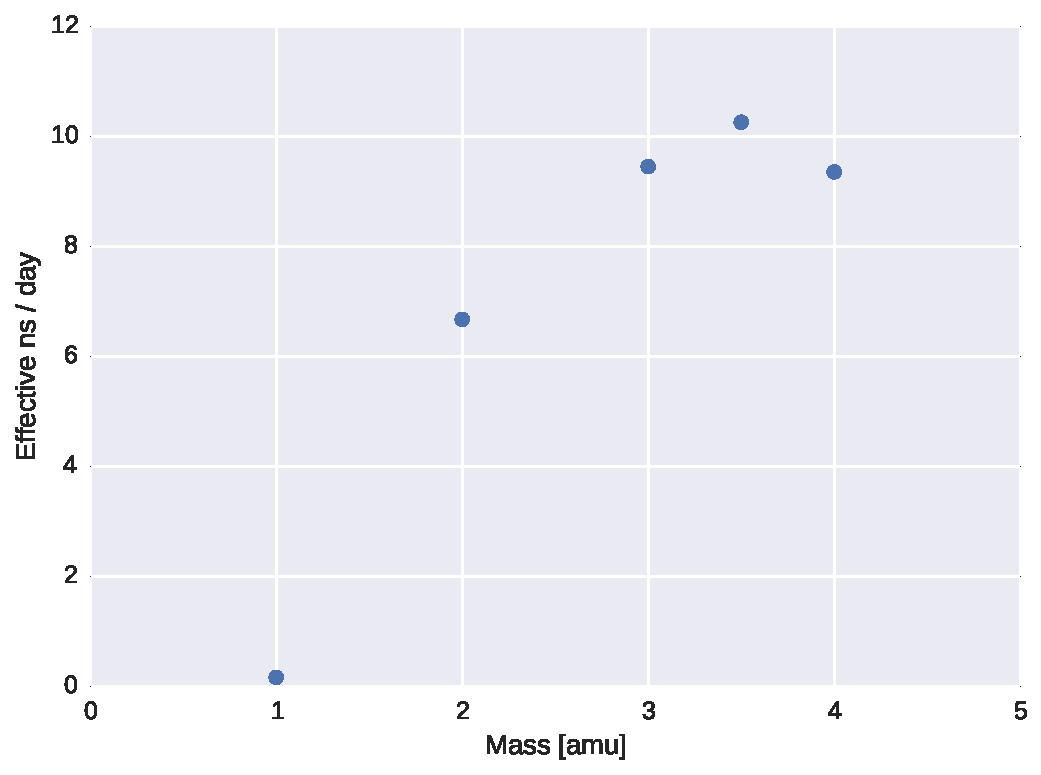
\includegraphics[width=\columnwidth]{./figures/hmr_masses.pdf}
\caption{{\bf HMR MASSES.}
The effect of hydrogen mass repartitioning on the effective performance, as measured by the raw performance times the acceptance rate.
}
\label{figure:hmr_masses}
\end{figure}


\subsection{Choice of steps per HMC iteration}

\subsection{Multiple Timestep GHMC: MTSGHMC}

\subsection{Alanine Populations and escape times}

\subsection{XCGHMC and XCMTSGHMC}

\subsection{Raw Performance: The cost of fancy integrators}

\begin{table}
\begin{tabular}{lr}
\toprule
{} & ns\_per\_day \\
\midrule
name        &            \\
vvvr        &       90.7 \\
ghmc1       &       33.7 \\
ghmc10      &       82.7 \\
vv          &       91.7 \\
ghmcrespa20 &       69.8 \\
verlet      &      103.7 \\
ghmc20      &       90.7 \\
langevin    &      103.9 \\
\bottomrule
\end{tabular}
\caption{{\bf Raw Performance of Various Integrators}
Raw performance on DHFR, assuming a 2 fs timestep. This does NOT incorporate the acceptance rate.
}
\label{table:ThermoMLSummary}
\end{table}





\section{Conclusions}

Density 

%%%%%%%%%%%%%%%%%%%%%%%%%%%%%%%%%%%%%%%%%%%%%%%%%%%%%%%%%%%%%%%%%%%%%%%%%%%%%%%%
% ACKNOWLEDGMENTS
%%%%%%%%%%%%%%%%%%%%%%%%%%%%%%%%%%%%%%%%%%%%%%%%%%%%%%%%%%%%%%%%%%%%%%%%%%%%%%%%

\section{Acknowledgements}

We thank Patrick B.~Grinaway (MSKCC), Vijay S.~Pande (Stanford University), Lee-Ping Wang (Stanford University), Peter Eastman (Stanford University), Robert McGibbon (Stanford University), Jason Swails (Rutgers University), David L.~Mobley (University of California, Irvine), Christopher I.~Bayly (OpenEye Software), Michael R. Shirts (University of Virginia), and members of Chodera lab for helpful discussions.  
Support for JMB was provided by the Tri-Institutional Training Program in Computational Biology and Medicine (via NIH training grant 1T32GM083937).  KAB was supported in part by Starr Foundation grant I8-A8-058.  JDC and KAB acknowledge partial support from NIH grant P30 CA008748.  KAB, JLB, ASR, and JDC acknowledge the generous support of this research by the Sloan Kettering Institute.

%%%%%%%%%%%%%%%%%%%%%%%%%%%%%%%%%%%%%%%%%%%%%%%%%%%%%%%%%%%%%%%%%%%%%%%%%%%%%%%%
% DISCLAIMERS
%%%%%%%%%%%%%%%%%%%%%%%%%%%%%%%%%%%%%%%%%%%%%%%%%%%%%%%%%%%%%%%%%%%%%%%%%%%%%%%%

\bibliography{benchmark}

\end{document}
